
\documentclass{article}
\usepackage{listings}
\usepackage{graphicx}
\usepackage[slovene]{babel}
\usepackage{color}
\usepackage{amsmath}
\usepackage[usenames,dvipsnames]{xcolor}
\usepackage[hidelinks]{hyperref}
\usepackage{subcaption}
\usepackage{float}
\usepackage{rotating} 
\usepackage{hyperref}
\usepackage{caption}
\graphicspath{{./images/}}

\setlength{\parindent}{0pt}

\newcommand{\MAD}{\mathrm{MAD}}


\begin{document}

\title{Matematično-fizikalni praktikum \\[3mm] \large Naloga 4}
\author{Luka Papež}
\date{12.\ november 2024}

\begin{center}
    
\includegraphics[width=8cm]{logo-fmf.png}
\end{center}

{
    \let\newpage\relax
    \maketitle
}

\maketitle
\newpage
\section{Naloga}

\begin{enumerate}
\item Izračunaj Fourierov obrat Gaussove porazdelitve in nekaj enostavnih vzorcev,
npr. mešanic izbranih frekvenc. Za slednje primerjaj rezultate, ko
je vzorec v intervalu periodičen (izbrane frekvence so mnogokratniki
osnovne frekvence), z rezultati, ko vzorec ni periodičen (kako naredimo Gaussovo porazdelitev `periodično' za FT?).
Opazuj pojav potujitve na vzorcu, ki vsebuje frekvence nad Nyquistovo
frekvenco. Napravi še obratno transformacijo in preveri
natančnost metode. Poglej, kaj se dogaja z časom računanja - kako je odvisen od števila vzorčenj?
\item Po Fourieru analiziraj \SI{2.3}{s} dolge zapise začetka Bachove
partite za violino solo, ki jih najdeš na spletni strani
Matematičnofizikalnega praktikuma.  Signal iz začetnih taktov
partite je bil vzorčen pri \SI{44100}{Hz}, \SI{11025}{Hz}, \SI{5512}{Hz}, \SI{2756}{Hz},
\SI{1378}{Hz} in \SI{882}{Hz}.  S poslušanjem zapisov v formatu {\tt .mp3}
ugotovi, kaj se dogaja, ko se znižuje frekvenca vzorčenja,
nato pa s Fourierovo analizo zapisov v formatu {\tt .txt}
to tudi prikaži.
\item \textbf{Dodatno:} Napravi Fourierovo analizo signalov, ki jih dobiš pri vaji
{\sl Akustični resonator\/} pri Fizikalnem praktikumu II.
Posnetke treh različnih signalov prav tako najdeš na spletni strani.
\end{enumerate}

\section{Uvod}

Pri numeričnem izračunavanju Fourierove transformacije
\begin{equation}
H(f) = \int_{-\infty}^\infty
h(t)\exp(2 \pi \ii f t)\dd t
\label{eq:ft}
\end{equation}
\begin{equation}
h(t) = \int_{-\infty}^\infty
H(f)\exp(-2 \pi \ii f t)\dd f
\end{equation}
je funkcija $h(t)$ običajno predstavljena s tablico diskretnih
vrednosti
\begin{equation}
  h_k = h(t_k),\quad t_k = k \Delta, \quad k=0,1,2,\dots N-1.
  \label{eq:discrete}
\end{equation}
Pravimo, da smo funkcijo vzorčili z vzorčno gostoto (frekvenco) $f=1/\Delta$.
Za tako definiran vzorec obstaja naravna meja frekvenčnega spektra,
ki se imenuje {\sl Nyquistova frekvenca}, $f_c =1/(2\Delta)$:
harmonični val s to frekvenco ima v vzorčni gostoti ravno
dva vzorca v periodi.
če ima funkcija $h(t)$ frekvenčni spekter omejen na interval
$[-f_c, f_c ]$, potem ji z vzorčenjem nismo odvzeli nič informacije,
kadar pa se spekter razteza izven intervala, pride do {\sl potujitve\/}
({\sl aliasing\/}), ko se zunanji del spektra preslika v interval.

Frekvenčni spekter vzorčene funkcije (\ref{eq:discrete}) računamo samo
v $N$ točkah, če hočemo, da se ohrani količina informacije.
Vpeljemo vsoto
\begin{equation}
H_n = \sum_{k=0}^{N-1}
h_k \exp(2 \pi \ii k n / N),
\qquad n=-\tfrac{N}{2},\dots ,\tfrac{N}{2},
\label{eq:dft}
\end{equation}
ki jo imenujemo diskretna Fourierova transformacija
in je povezana s funkcijo v (\ref{eq:ft}) takole:
\begin{equation*}
H(\tfrac{n}{N\Delta}) \approx \Delta\cdot H_n .
\end{equation*}
Zaradi potujitve, po kateri je $H_{-n} = H_{N-n}$, lahko pustimo
indeks $n$ v enačbi (\ref{eq:dft}) teči tudi od 0 do $N$. Spodnja polovica
tako definiranega spektra ($1 \le n \le \tfrac{N}{2}-1$) ustreza pozitivnim
frekvencam $0 < f < f_c$, gornja polovica ($\tfrac{N}{2}+1 \le N-1$)
pa negativnim, $-f_c < f < 0$.  Posebna vrednost pri $n=0$
ustreza frekvenci nič (``istosmerna komponenta''), vrednost
pri $n=N/2$ pa ustreza tako $f_c$ kot $-f_c$.

Količine $h$ in $H$ so v splošnem kompleksne, simetrija
v enih povzroči tudi simetrijo v drugih.  Posebej zanimivi
so trije primeri:\par\medskip
\begin{tabular}{@{\hspace{1cm}}l@{\hspace{1cm}}l@{\hspace{1cm}}l@{\hspace{1cm}}l}
če je& $h_k$ realna & tedaj je & $H_{N-n} = H_n^\ast$ \\
      & $h_k$ realna in soda & & $H_n$ realna in soda \\
      & $h_k$ realna in liha & & $H_n$ imaginarna in liha
\end{tabular}
\par\medskip
(ostalih ni težko izpeljati).
V tesni zvezi s frekvenčnim spektrom je tudi moč.
{\sl Celotna moč\/} nekega signala je neodvisna od
reprezentacije, Parsevalova enačba pove
\begin{equation*}
\sum_{k=0}^{N-1} | h_k |^2 = {1\over N}\sum_{n=0}^{N-1} | H_n |^2
\end{equation*}
(lahko preveriš).  Pogosto pa nas bolj zanima, koliko moči
je vsebovane v frekvenčni komponenti med $f$ in $f+\dd f$, zato
definiramo enostransko spektralno gostoto moči ({\sl one-sided
power spectral density\/}, PSD)
\begin{equation*}
P_n = | H_n |^2 + | H_{N-n} |^2 \>.
\end{equation*}
Pozor: s takšno definicijo v isti koš mečemo negativne
in pozitivne frekvence, vendar sta pri realnih signalih $h_k$
prispevka enaka, tako da je $P_n = 2\,| H_n |^2$.

Z obratno transformacijo lahko tudi rekonstruiramo $h_k$ iz $H_n$
\begin{equation}
  h_k = {1\over N} \sum_{n=0}^{N-1} H_n \exp(-2 \pi \ii k n / N)
  \label{eq:inverz}
\end{equation}
(razlika glede na enačbo je le predznak v argumentu
eksponenta in utež $1/N$).
\newpage
\section{Rešitev}
\subsection{Fourirjeva transformacija osnovnih funkcij}
K nalogi pristopim s fourirjevo transformacijo(FT) nekaj osnovnih funkcij. S pomočjo katerih se bomo spoznali z njihovim delovanjem preden se lotimo preostalih bolj zakompliciranih delov naloge.
Za začetek si poglejmo FT vsote sinusnih funkcij. FT nam bo vrnila amplitude sinusnih funkcij pri x koordinati, ki predstavlja njihovo frekvenco. 
\begin{figure}[H]
    \centering
    \begin{minipage}{0.48\textwidth}
        \centering
        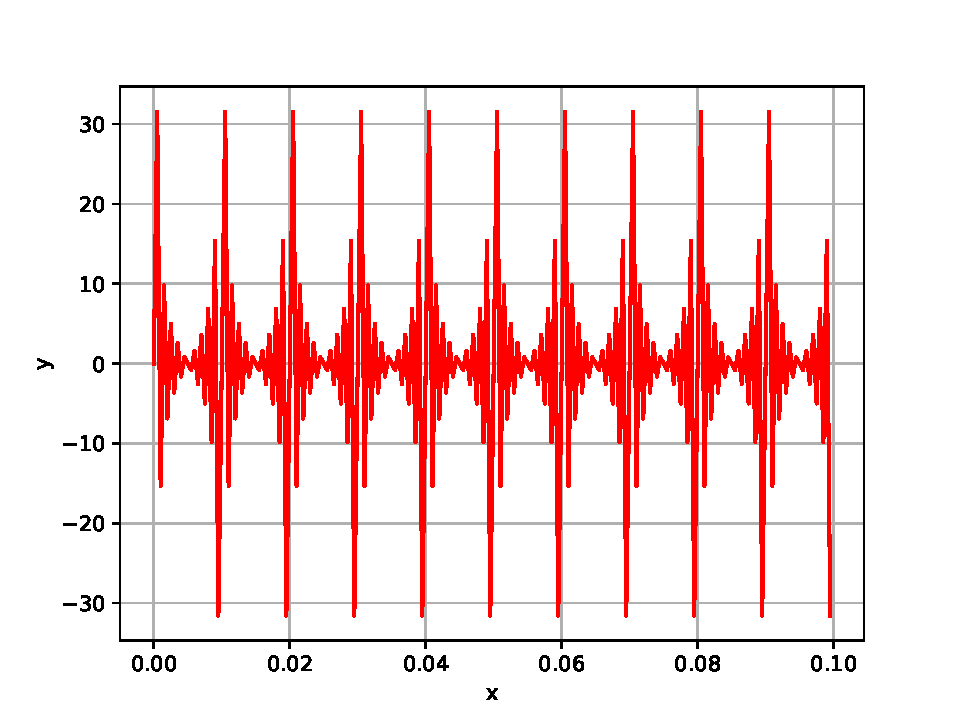
\includegraphics[width=\textwidth]{sinefunc.pdf}
        \caption{Transformirana vsota sinusnih funkcij}
    \end{minipage}
    \hfill
    \begin{minipage}{0.48\textwidth}
        \centering
        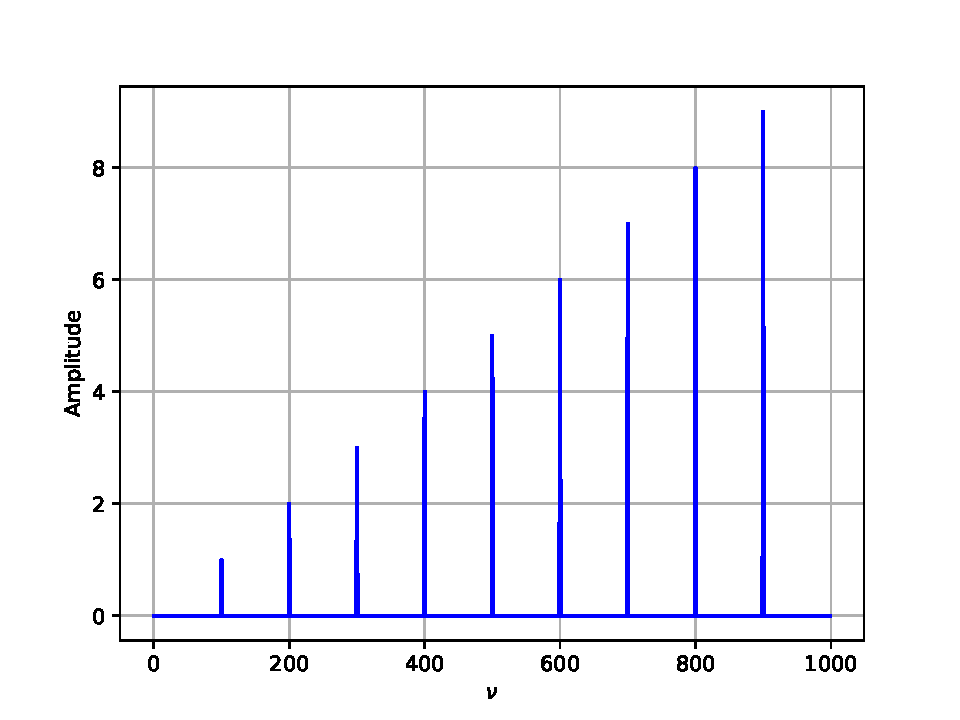
\includegraphics[width=\textwidth]{sines.pdf}
        \caption{FT vsote sinusov z amplitudo, ki je stotina njihove frekvence}
    \end{minipage}
\end{figure}

Po FT dobimo pričakovane vrednosti glede na vhodne podatke. Iz grafa jasno razberemo frekvence, ki so večkratniki števila $100k (k \in [0, 9])$. Vidimo pa tudi linearno naraščanje amplitud, ki so stotina frekvence funkcije.
Dobljene delte funkcije pa lahko izkoristimo za preizkus natančnosti inverzne fourirjeve transformacije(IFT). Kot rezultat dobimo funkcijo, ki ima odstopanja reda $O(-14)$. S čemer smo pokazali, da je na tem primeru IFT zelo natančen. Poglejmo si še primer FT delta funkcija in vsote nekaj delt funkcij.

\begin{figure}[H]
    \centering
    \begin{minipage}{0.48\textwidth}
        \centering
        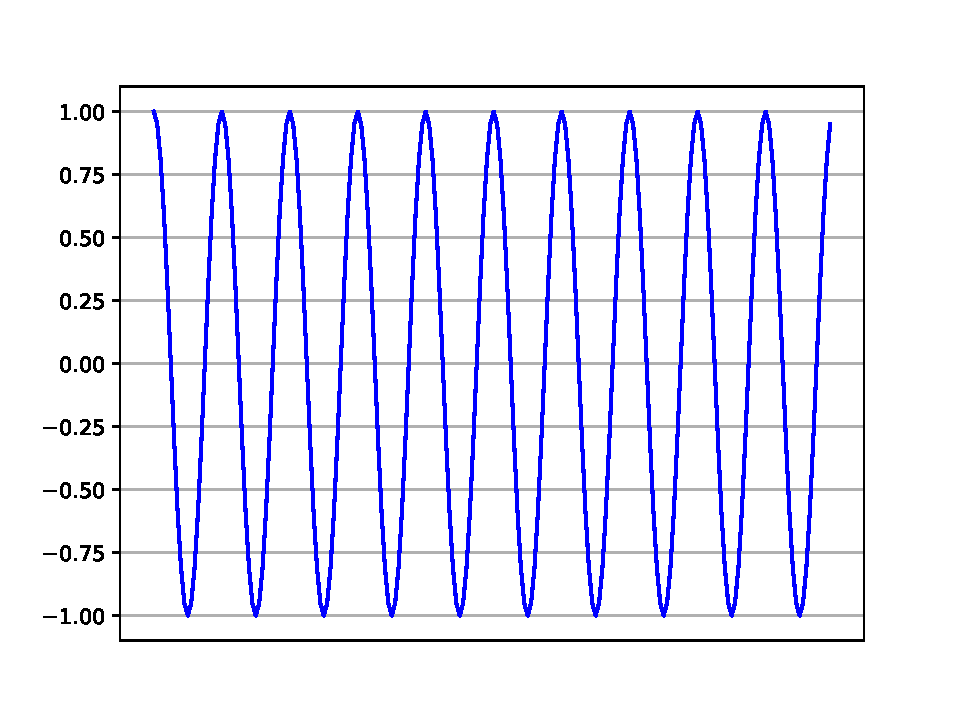
\includegraphics[width=\textwidth]{deltasingle.pdf}
		\caption{Transformiranka $\delta(x - 10)$}
    \end{minipage}
    \hfill
    \begin{minipage}{0.48\textwidth}
        \centering
        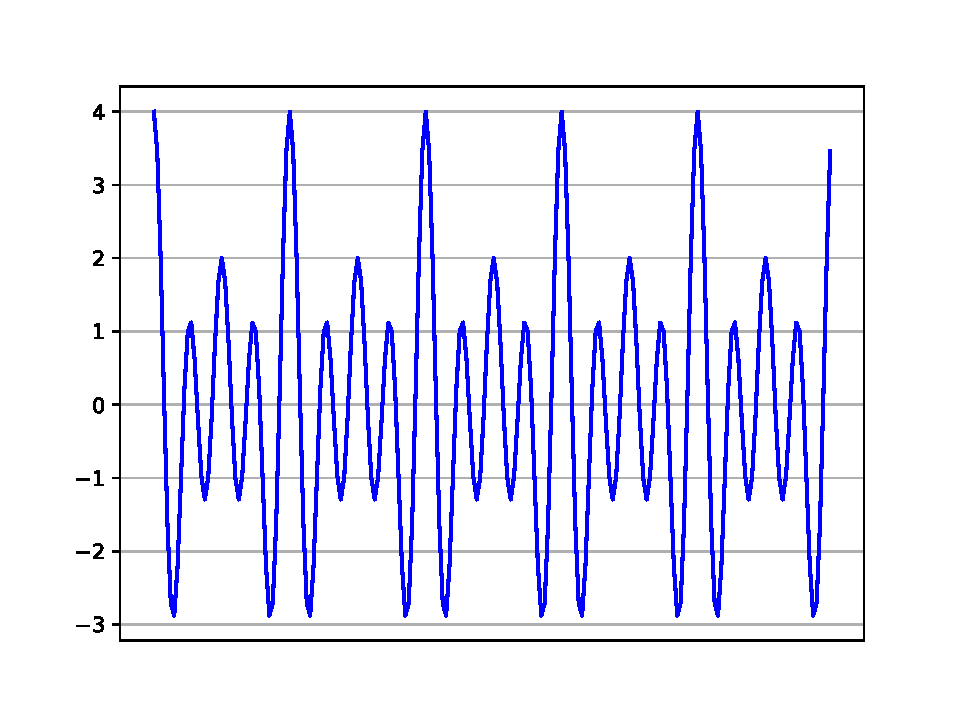
\includegraphics[width=\textwidth]{delta.pdf}
		\caption{Transformiranka $\delta(x - 10) + \delta(x - 15) + \delta(x -20)$ }
    \end{minipage}
\end{figure}
V kontekstu FT je zanimiva tudi Gaussove funkcija, saj je njena transformiranka tudi Gaussova funkcija. Za primer bomo vzeli rahlo poenostavljeno obliko $e^{-ax^2}$ katere rezultat FT je splošno znan:
\begin{equation*}
	\sqrt{\frac{\pi}{a}} e^{-\frac{\pi^2 k^2}{a}}
\end{equation*}
\begin{figure}[H]
    \centering
    \begin{minipage}{0.48\textwidth}
        \centering
        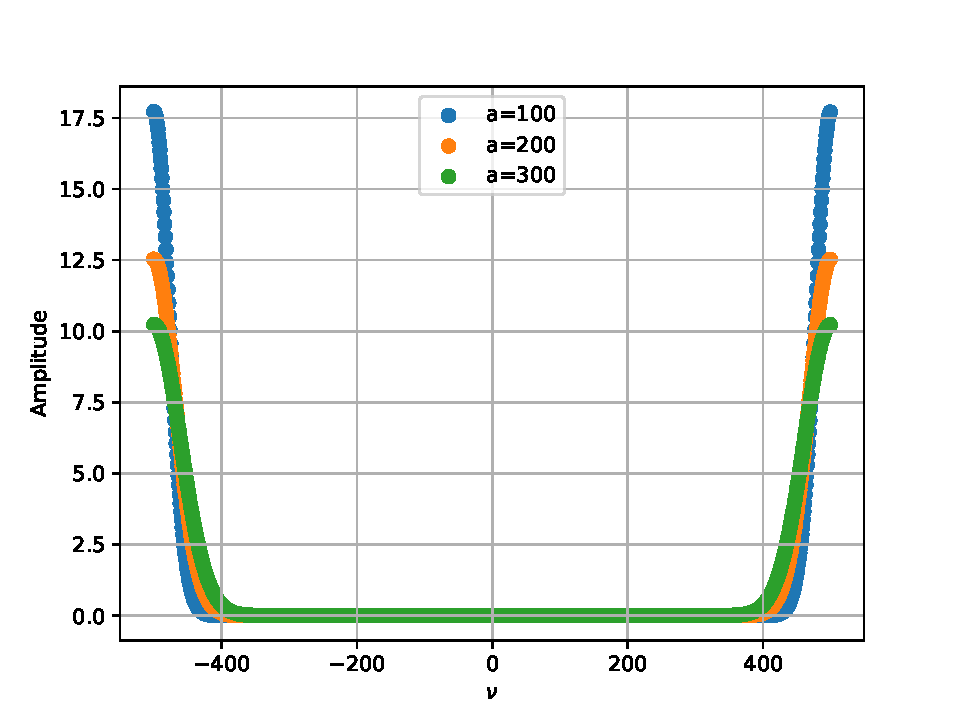
\includegraphics[width=\textwidth]{nomirrorgauss.pdf}
		\caption{FT poenostavljene Gaussove funkcije $e^{-ax^2}$ pri različnih vrednostih a}
		\label{slika5}
    \end{minipage}
    \hfill
    \begin{minipage}{0.48\textwidth}
        \centering
        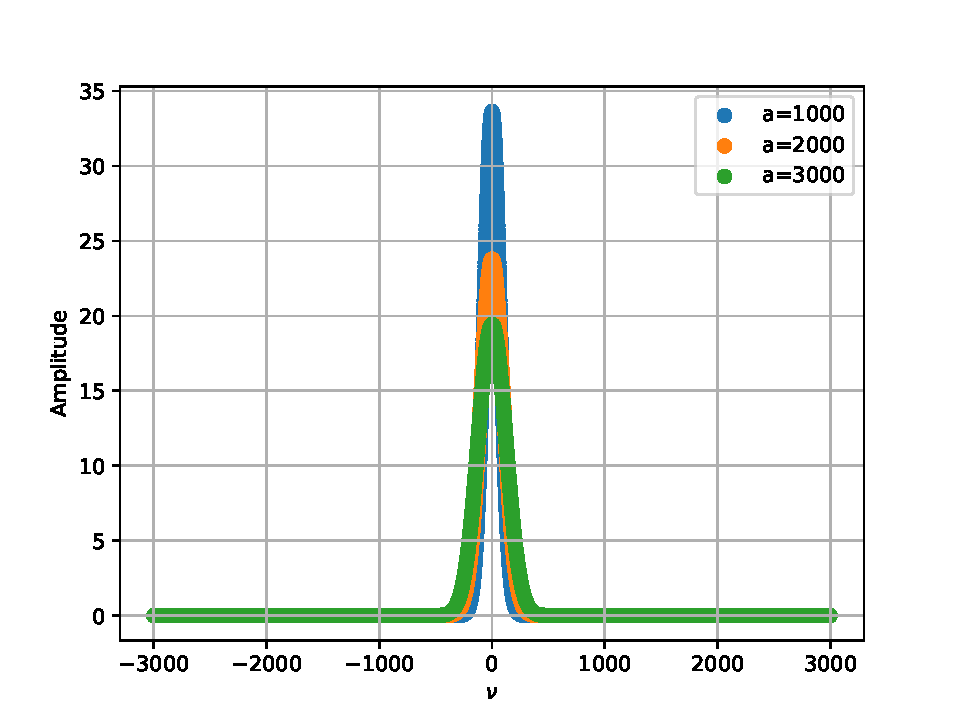
\includegraphics[width=\textwidth]{gauss.pdf}
	\caption{FT poenostavljene Gaussove funkcije $e^{-ax^2}$ pri različnih vrednostih a z zrcaljenjem}
		\label{slika6}
    \end{minipage}
\end{figure}
Najprej dobimo nenavaden rezultat na sliki \ref{slika5}. Razlog za njim je ne periodičnost Gaussove funkcije. Zato, da dosežemo periodičnost Gaussovo funkcijo zrcalimo. Tako dobimo pričakovan rezultat, ki je na sliki \ref{slika6}.
\subsection{Nyquistova frekvenca in časovna odvisnost računanja FT}
Kot že omenjeno v uvodu Nyquistova frekvenca označuje kritično točko, kjer je frekvenca vzorčenja premajhna za frekvence v našem signalu. Po tej točki pa se pojavi pojav imenovan `aliasing`. Da prikažemo ta pojav vzamemo za primer signal $\sin(2 \pi 20t) + \sin(2\pi 100 t)$.
\begin{figure}[H]
    \centering
	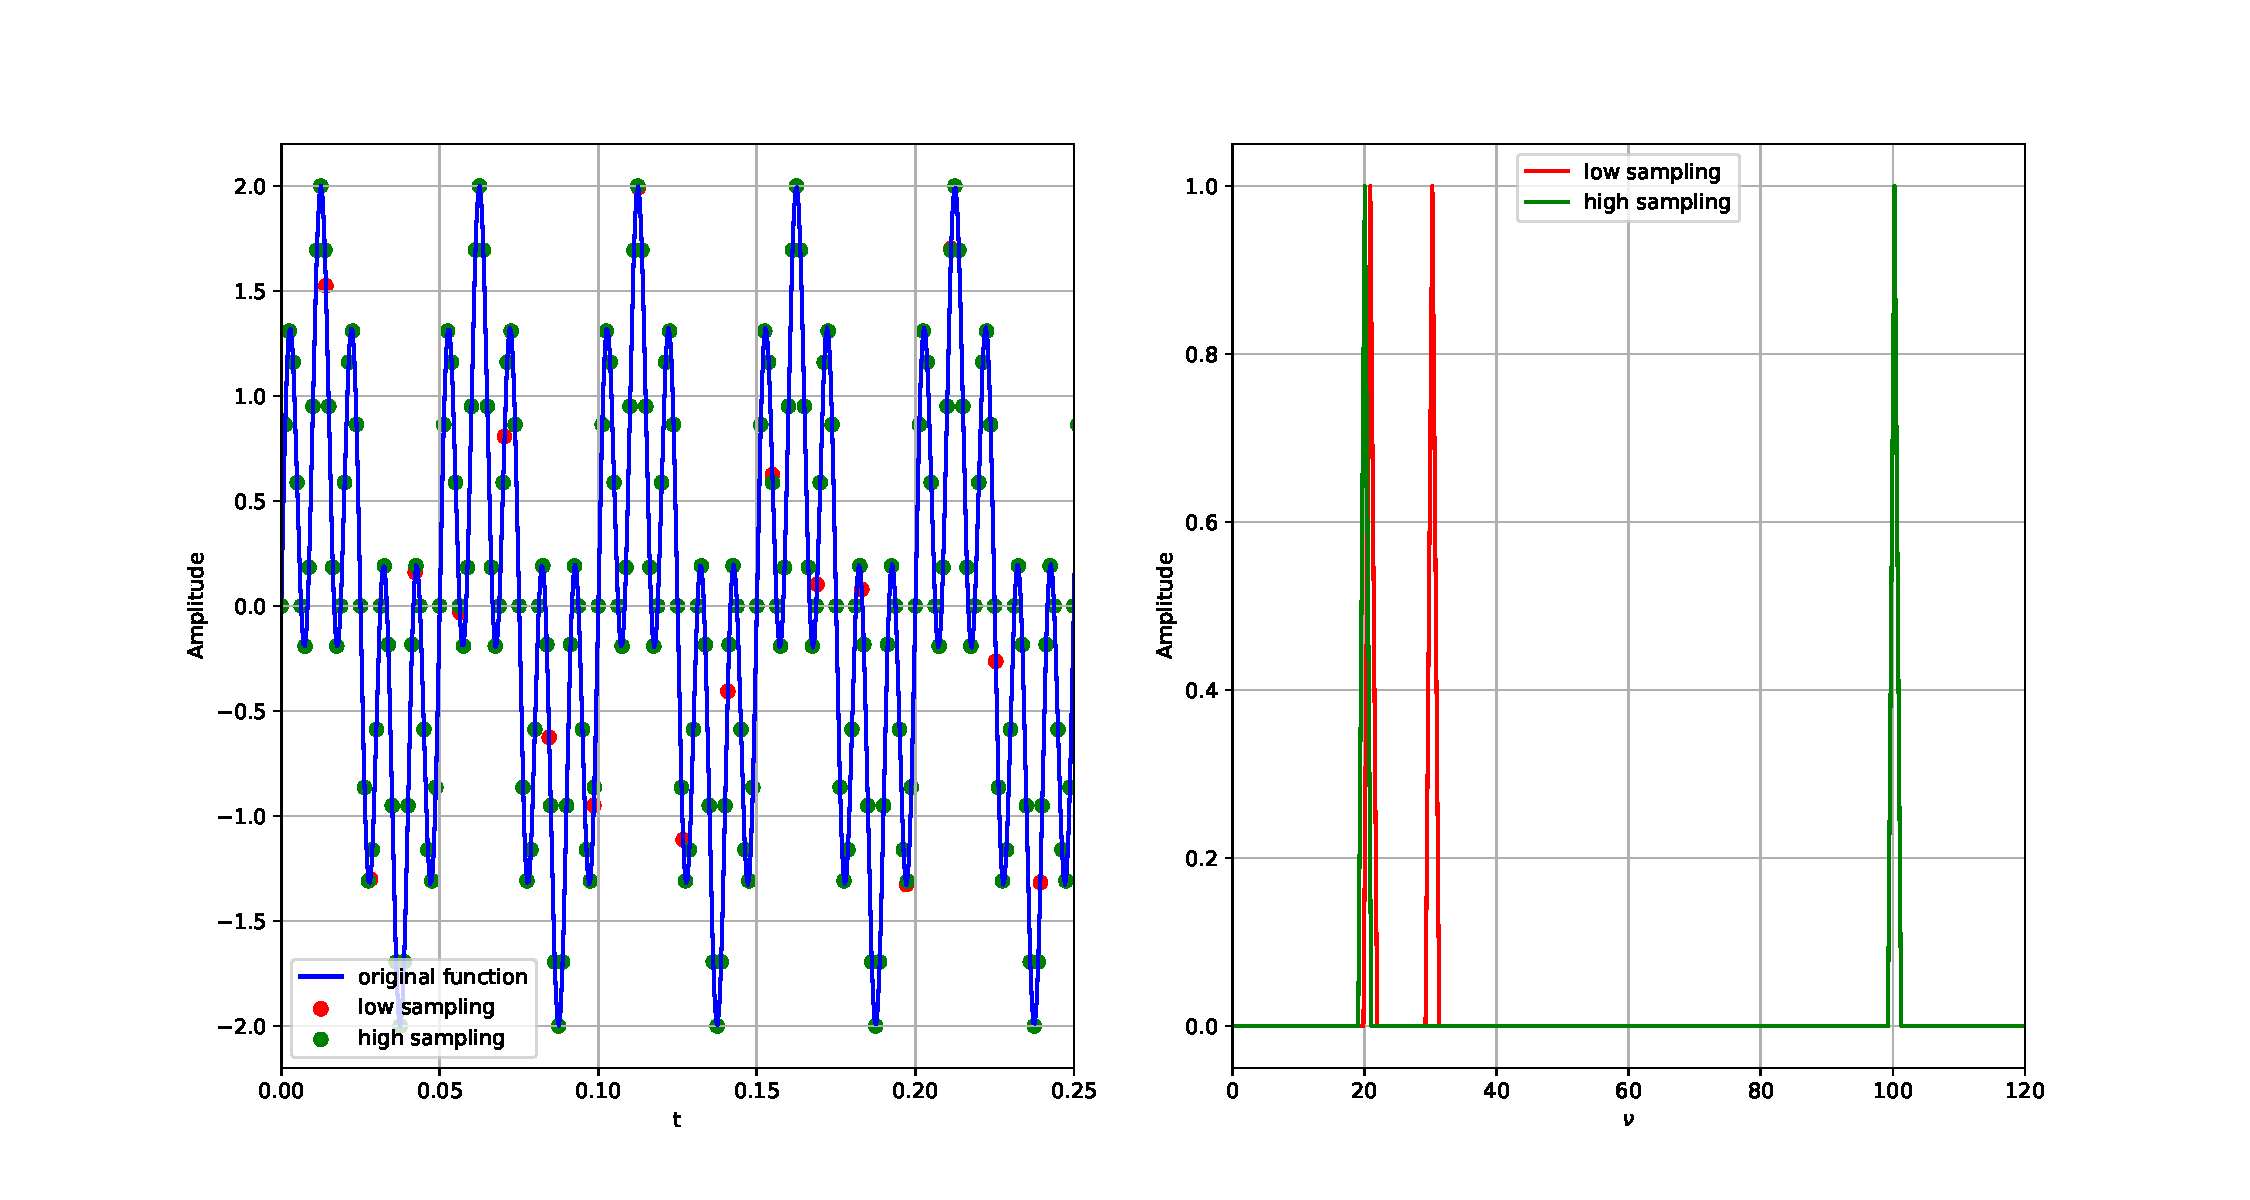
\includegraphics[width=1\textwidth]{nyquist.pdf}
    \caption{Primer aliasing. Na desni sliki je prikaz vzorčenja signala in na desni FT za vsak sampling}
\end{figure}
Z našim primerom smo uspešno pokazali pojav `aliasing`. Saj se je pri manjšem vzorčenju druga frekvenca pojavila pri približno 30. Kasneje pa se je pri primernem vzorčenju izkazala prava vrednost. Medtem ko se vrednosti manjše frekvence praktično prekrivata. Na tem primeru pa si poglejmo še kako se obnaša časovna zahtevnost podanih funckij diskretne Fourirjeve transformacije(DFT) in še vgrajeni funkciji hitre Fourirjeve transformacije(FFT) iz knjižnic `cupy` in `numpy`.
\begin{figure}[H]
    \centering
    \begin{minipage}{0.48\textwidth}
        \centering
        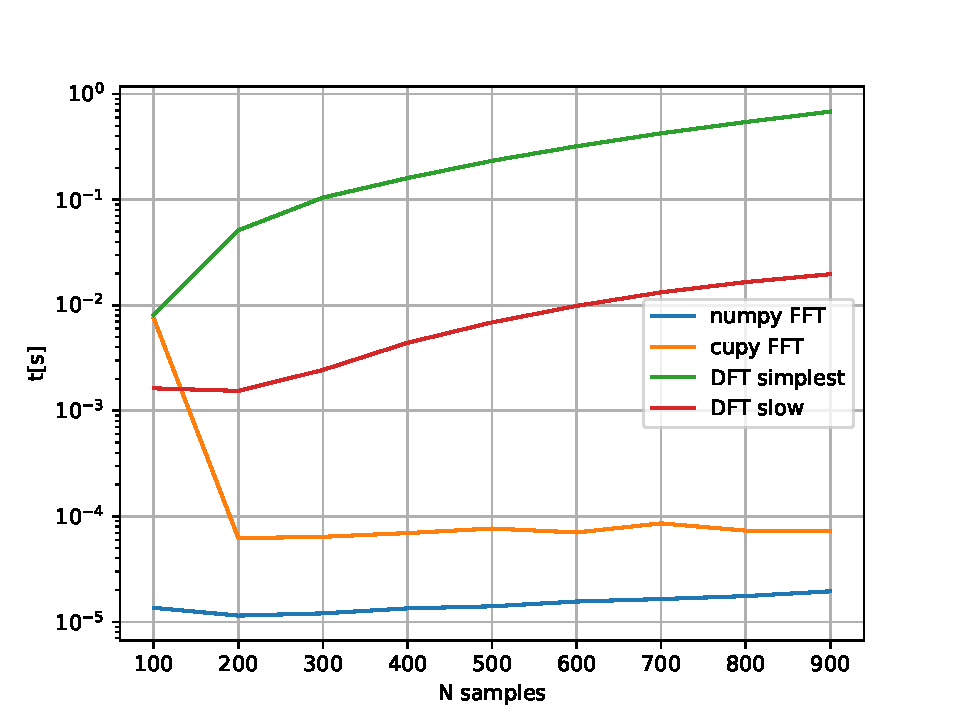
\includegraphics[width=\textwidth]{dtf.pdf}
		\caption{Hitrost funkcij diskretne Fourirjeve transofrmacije in vgrajenih funkcij hitre Fourirjeve transformacije}
		\label{slika5}
    \end{minipage}
    \hfill
    \begin{minipage}{0.48\textwidth}
        \centering
        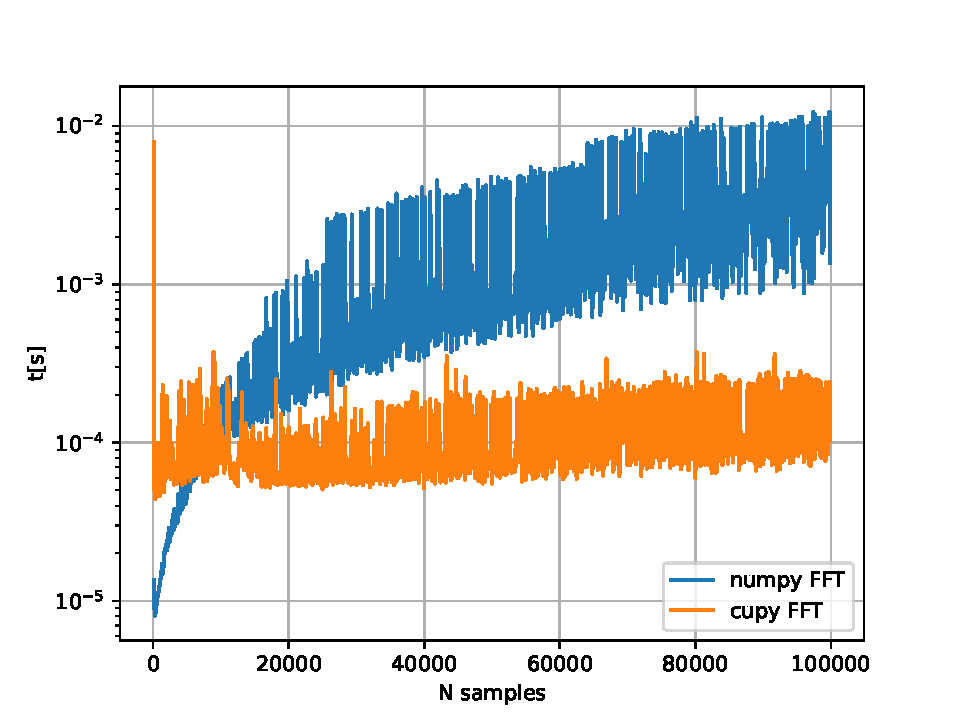
\includegraphics[width=\textwidth]{cupynumpy.pdf}
		\caption{Hitrost vgrajenih funkcij hitre Fourirjeve transformacije}
		\label{slika6}
    \end{minipage}
\end{figure}
Kot pričakovano sta funkciji precej počasnejši od vgrajenih funkcij FFT. Zato je drug graf precej bolj zanimiv. Najprej opazimo dejstvo, da kljub temu, da smo povprečili vrednosti desetih izračunov so vrednosti zelo nestabilne. Poleg tega ima knjižnica, ki uporablja grafično kartico, čez vsa števila vzorčenja približno enak čas izračuna. To namiguje, da s preizkušenimi vrednostmi nismo uspeli popolnoma izkoristiti njene hitrosti in prevladuje nek drug faktor kot je na primer prenos podatkov na grafično kartico. Hitrost računanja na procesorju pa je na začetku precej hitrejša od ekvivalenta na grafični kartici. Z naraščanjem števila vzorcev pa postane precej počasnejša. 
\subsection{Bachove partite}
Drugi del naloge pa je analiza prvih 2.6s Bachove partite za violino solo. Iz poslušanja posnetkov sem osebno razbral, da počasi predvsem od $5512Hz$ naprej začnejo izginjati višje frekvence. Bolj opisno je zadnji posnetek zvenel kot, da bi ga poslušal pod vodo. 
\\\\
FT različnih vzorčenj Bachove partite so na voljo na naslednji strani. Iz njih je razvidno, da v posnetku prevladuje frekvenca pri približno $250Hz$. Če se za trenutek spomnimo Nyquistove frekvence z njo lahko potrdimo, da je že spekter pri $5512Hz$ precej dober. Kar se nekako tudi ujema z našo ugotovitvijo iz poslušanja. Dejstvo, da z nižjim vzorčenjem izgubljamo informacije o višjih frekvencah pa tudi pojasni zakaj se v posnetkih zdi, da višje frekvence izginjajo. 
\begin{figure}[H]
    \centering
	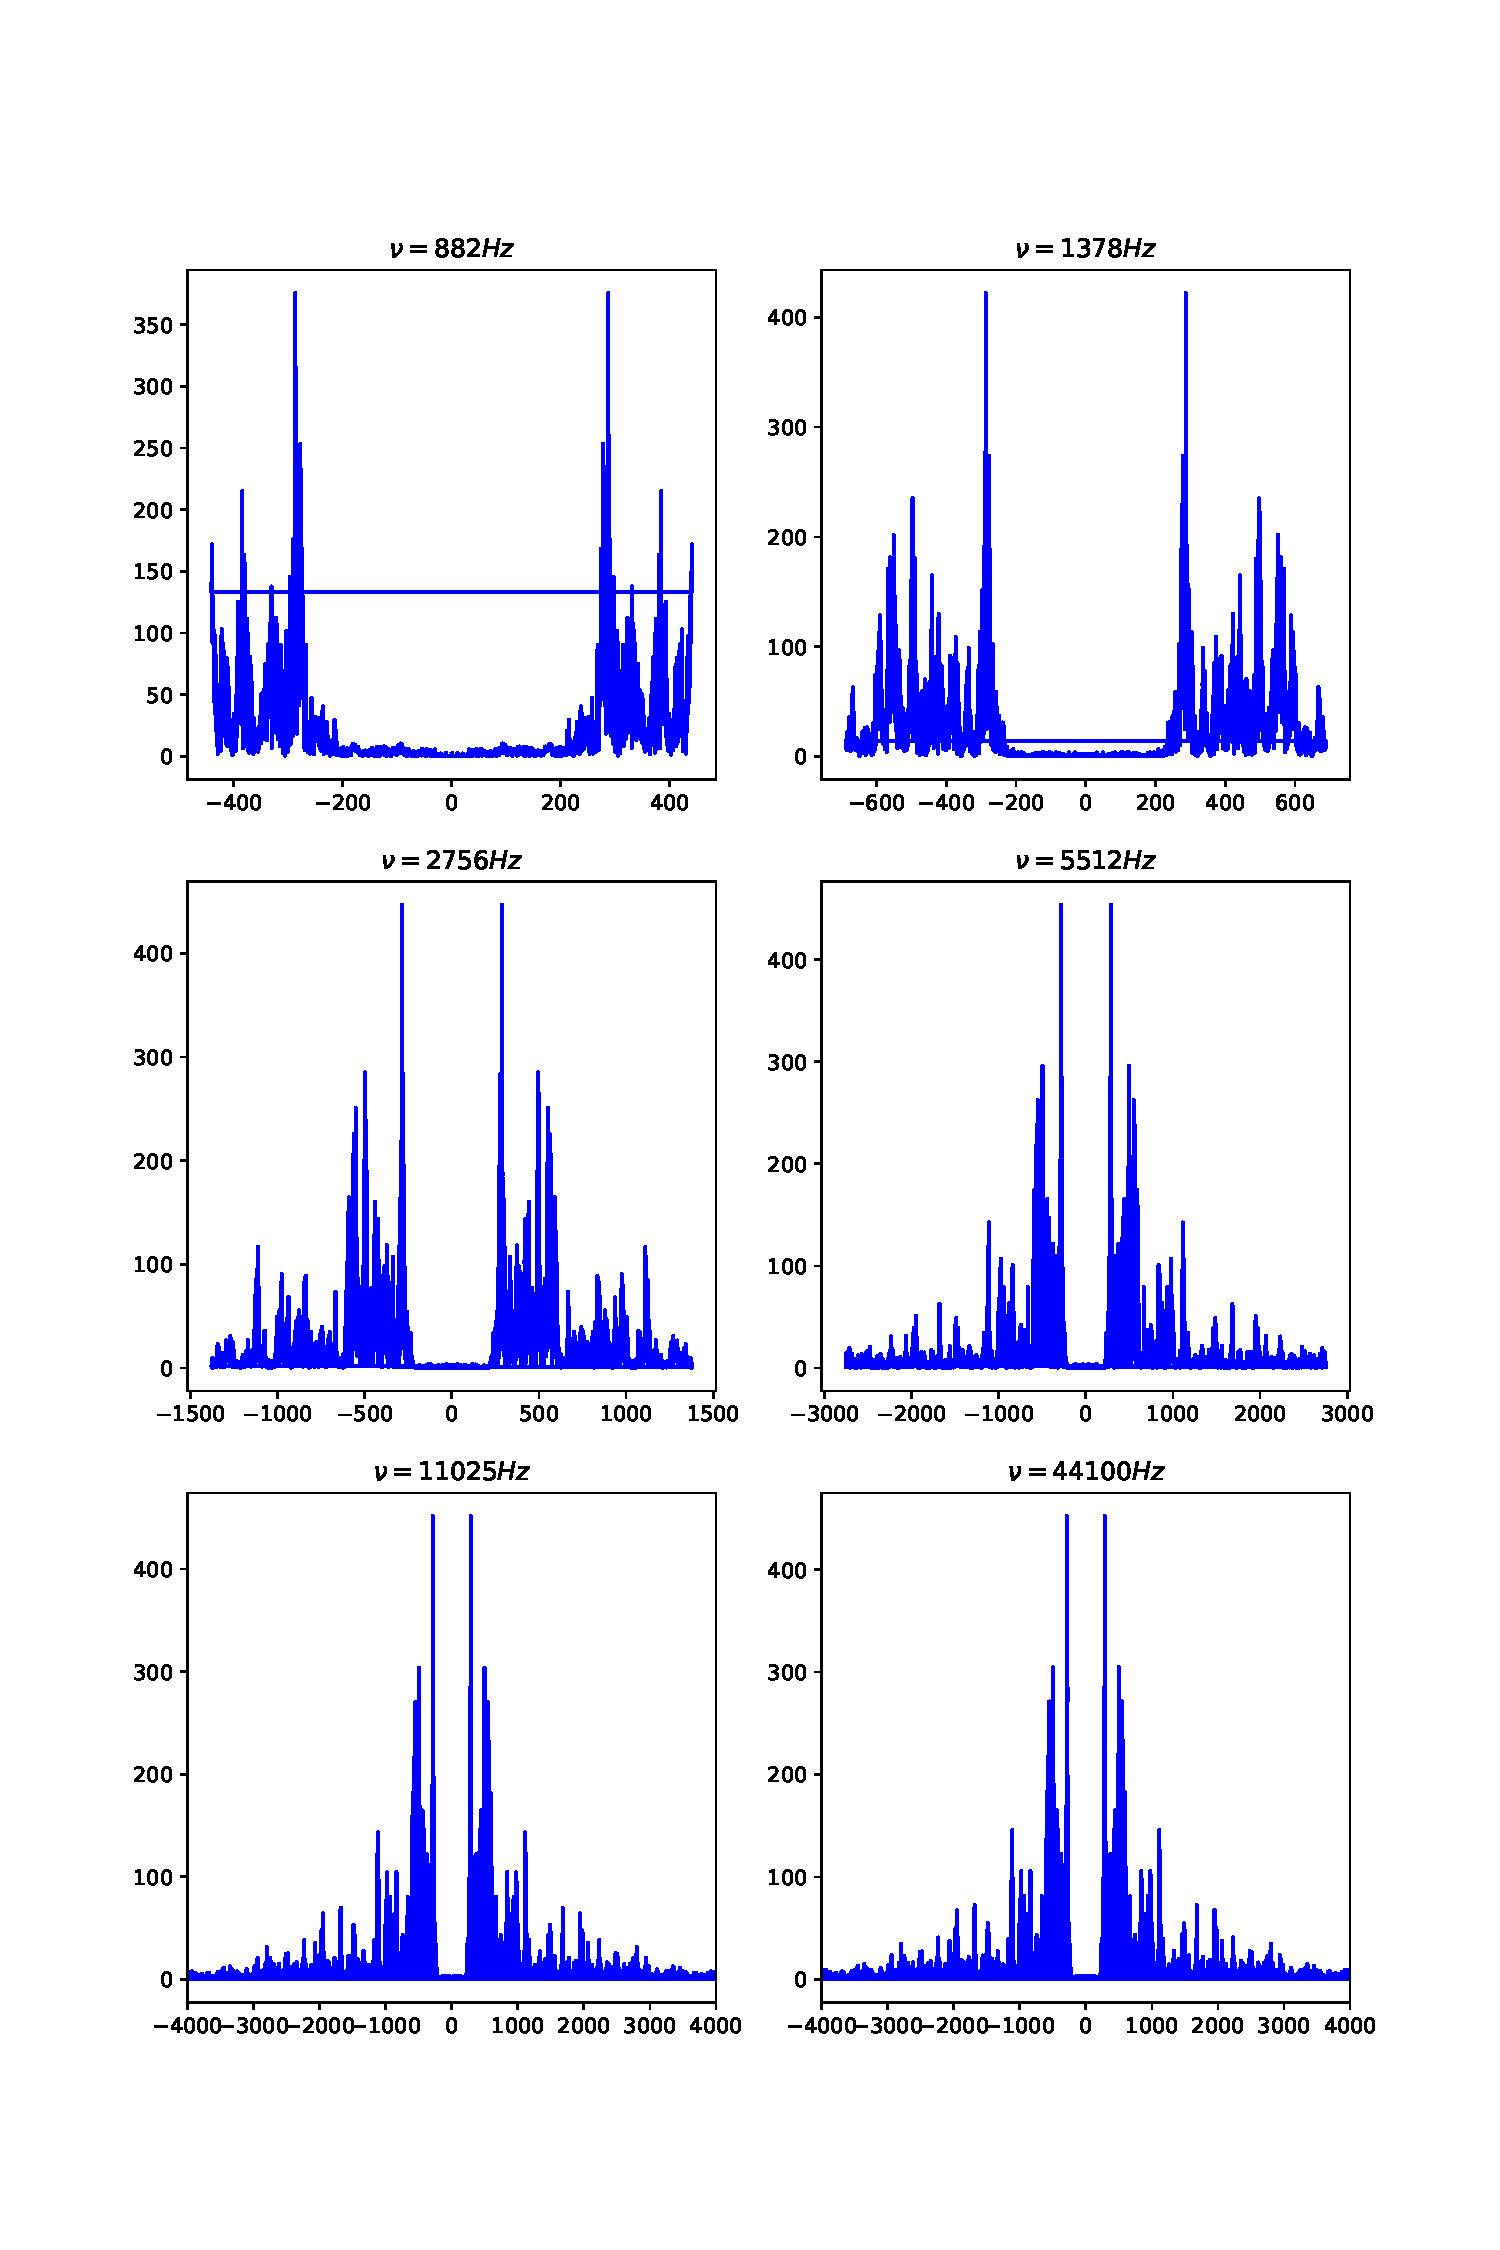
\includegraphics[width=1\textwidth]{bach.pdf}
	\caption{FT Bachove partite za violino solo}
\end{figure}
\section{Zaključek}
Naloga je bila precej drugačna od ostali do sedaj in se je osredotočila na razumevanje obnašanja Fourirjeve transformacije in težav, ki nastopijo pri njej. Fourirjeva transformacija ima tudi precej uporab, zato prilagam \href{https://www.youtube.com/watch?v=GGPjQGOCbTY}{povezavo do videa z zanimivo uporabo}. 
\end{document}
